\documentclass[runningheads]{llncs}
\usepackage[utf8]{inputenc}
%\usepackage[top=1in, bottom=1in, left=1in, right=1in]{geometry}
% \usepackage{times}
\usepackage{amsmath}
\usepackage{graphicx}
%\usepackage{setspace}
%\usepackage{subfig}
%\usepackage[hyphens]{url}
\usepackage{hyperref}
\usepackage{xspace}
\usepackage{color}
\usepackage{forest}
\usetikzlibrary{backgrounds,fit,positioning}
%\usepackage{flushend}
\usepackage{paralist}
\usepackage[ruled,vlined]{algorithm2e}
\usepackage{enumitem}

\usepackage{caption}
\usepackage{tabularx}
\usepackage{booktabs}
\usepackage{amssymb}
\usepackage[]{todonotes}

  
\newcommand{\sys}{Promise\xspace}
\newcommand{\discount}{\sum_{t=0}^{T} \big( \frac{\delta}{1+r} \big)^t}

\newcommand{\todoin}[1]{\todo[inline,caption={}]{#1}}
\newcommand{\toall}[1]{\todo[linecolor=orange,backgroundcolor=orange!25,bordercolor=orange,inline, caption={}]{Unassigned Todo: #1}}

\newcommand{\aza}[1]{\todo[linecolor=blue,backgroundcolor=blue!25,bordercolor=blue,inline,caption={}]{Comment by Alexei: #1}}
\newcommand{\toaza}[1]{\todo[linecolor=blue,backgroundcolor=blue!25,bordercolor=blue,inline,caption={}]{Todo for Alexei: #1}}

\newcommand{\rk}[1]{\todo[linecolor=red,backgroundcolor=red!25,bordercolor=blue,inline,caption={}]{Comment by Rami: #1}}
\newcommand{\tork}[1]{\todo[linecolor=blue,backgroundcolor=red!25,bordercolor=red,inline,caption={}]{Todo for Rami: #1}}

\newcommand{\lgu}[1]{\todo[linecolor=yellow,backgroundcolor=yellow!25,bordercolor=yellow,inline,caption={}]{Comment by Lewis: #1}}
\newcommand{\tolgu}[1]{\todo[linecolor=yellow,backgroundcolor=yellow!25,bordercolor=yellow,inline,caption={}]{Todo for Lewis: #1}}

\newcommand{\dom}[1]{\todo[linecolor=green,backgroundcolor=green!25,bordercolor=green,inline,caption={}]{Comment by Dominik: #1}}
\newcommand{\todom}[1]{\todo[linecolor=green,backgroundcolor=green!25,bordercolor=green,inline,caption={}]{Todo for Dominik: #1}}

\begin{document}

\title{
\sys: Leveraging Future Gains for Collateral Reduction
% \sys: Leveraging Future Payments for Bootstrapping Collateralized Protocols
} 
\author{
Dominik Harz, Lewis Gudgeon, Rami Khalil, Alexei Zamyatin
\institute{
Department of Computing, Imperial College London}
}


\date{}
\maketitle

%-------------------------------------------------
%---------------ABSTRACT------------------------
%-------------------------------------------------

\begin{abstract}
% \dom{Proposal: change the paper to restrict the mechanism to protocols in which there is competition, i.e. Bob can exit when Alice is malicious. I think one of the biggest problems is that \sys does not work when you have a monopoly situation.}
Collateral employed in cryptoeconomic protocols protects against the misbehavior of economically rational agents, compensating honest users for damages and punishing misbehaving parties.
%It can increase the trustworthiness of a system by compensating honest users for damages and revoking the locked capital of cheating parties.
The introduction of collateral, however, carries three disadvantages: (i) requiring agents to lock up substantial amount of collateral can be an entry barrier, limiting the set of candidates to wealthy agents; (ii) affected agents incur ongoing opportunity costs as the collateral cannot be utilized elsewhere; and (iii) users wishing to interact with an agent on a frequent basis (e.g., with a service provider to facilitate second-layer payments), have to ensure the correctness of each interaction individually instead of subscribing to a service period in which interactions are secured by the underlying collateral.
%First, a substantial lockup requirement can act as a barrier to entry for certain protocol roles, limiting the set of candidates to wealthy agents.
%Second, agents incur ongoing opportunity costs while their collateral is locked up, as it cannot be utilized elsewhere.

We present \sys, a subscription mechanism to decrease the initial capital requirements of economically rational service providers in cryptoeconomic protocols.
The mechanism leverages future income (such as service fees) prepaid by users to reduce the collateral actively locked up by service providers, while sustaining secure operation of the protocol.
\sys is applicable in the context of multiple service providers competing for users.
We provide a model for evaluating its effectiveness and argue its security.
Demonstrating \sys's applicability, we discuss how \sys can be integrated into a cross-chain interoperability protocol, XCLAIM, and a second-layer scaling protocol, NOCUST.
Last, we present an implementation of the protocol on Ethereum showing that all functions of the protocol can be implemented in constant time complexity and \sys only adds USD 0.05 for a setup per user and service provider and USD 0.01 per service delivery during the subscription period.
% Lastly, we discuss how \sys can be applied to existing second-layer scaling, blockchain interoperability, and decentralized mining protocols.
%allowing the required collateral to be constituted by future transaction fees by the user, while \emph{sustaining the overall collateral} required as a security deposit.
%Using \sys, a user can force a service provider to lock payments as future collateral.
%Further, the user is able to provide multiple future payments in escrow to provide a revenue guarantee to a service provider.
%We show that, using \sys, delayed payments securely held in escrow can be fairly distributed after the predefined delay.
%We further argue that \sys motivates users to lock future payments as collateral and intermediaries have higher overall collateral.
% We further show that \sys leads to a Nash equilibrium where some agent roles are motivated to lock future payments as collateral to motivate other agent roles to behave honestly without degrading the overall security provided by a system.
%\dom{Do we need that layer-two mention in there? I think Promise as a scheme is also applicable to layer 1?}
%\rk{I removed the extra layer-two word. Does interop and decentralized mining count as pure L1?}
%\dom{I was wondering about mining pools (the non-decentralized ones). But I'm not sure. I also think in Bitcoin mining you delay the payout of the reward a couple of blocks by default because of the lack of finality. What do you think?}
%\rk{It's not exactly the same, because you can initiate a transfer from the miner's wallet to a recipient immediately in the next block, right? You can play "hot potato" with the mining reward.}
%Lastly, we elaborate on applying \sys to several commonly known protocols, including second-layer scaling, blockchain interoperability, and decentralized mining protocols.
%\rk{If we don't provide full example texts for things other than nocust then: Lastly, we elaborate on applying \sys to second-layer scaling.
%}
\end{abstract}

%-------------------------------------------------
%---------------INTRODUCTION------------------------
%-------------------------------------------------

\section{Introduction}
\label{sec:intro}

% \dom{TODO:
% \begin{itemize}
%     \item The intro should be 3/4 pages max
%     \item Make problem statement concise
%     \item clean up intuition
%     \item make sure assumptions are complete
% \end{itemize}}

Since their creation, arguably the most significant property of blockchains is their facilitation of trustless exchange between entities with weak identities~\cite{rainer}.%~\footnote{Agents with \emph{weak} identities are able to suddenly leave a network; agents with \emph{strong} identities cannot.}.
Yet the trustless nature of the systems means not only that parties \textit{may} transact without trusting each other, but also that they \textit{should not trust} each other.
%\footnote{Or at least should not trust each other.}.
This creates a design challenge for interactions which would typically involve such trust. 
% In this paper, we focus on blockchain protocols which, at least in part, express \textit{trust} through \textit{collateral}.
%Here, collateral is value escrowed by party A to guarantee party B that A will not misbehave given that A's economic gain from cheating is not higher than the collateral value.
% Here, collateral is value escrowed by party A to guarantee party B that regardless of the behavior of party A, party B cannot lose funds. 
In this paper, we focus on blockchain protocols which, at least in part, encode trust by monetary collateral.
%\dom{Definition is a bit tricky, would change that it not only relates to funds but basically under rationality assumption, A would not cheat.}
Here, collateral is value escrowed by a service provider, Alice, to guarantee the user, Bob, that regardless of the behavior of Alice, Bob cannot lose funds. 
%It allows us to create systems that are resistant against economically rational adversaries by imposing the threat of destroying their money and motivating their honest behavior.
In particular, payment, cross-chain, and generic computation protocols can be designed such that Bob is guaranteed to receive from Alice at least the amount of funds that are at risk in case she misbehaves.
Protocols involving collateral include cross-chain communication~\cite{Zamyatin2019XCLAIM}, scalable off-chain payments~\cite{Khalil2019NOCUST}, state channels~\cite{dziembowski2018general}, watchtowers~\cite{mccorry2018pisa,avarikioti2019brick,avarikioti2018towards}, and outsourcing of computation and verification games~\cite{teutsch2017scalable}

% Relying on collateral as a means of trust is associated with a different set of challenges. 
\paragraph{Problem.}
Relying on collateral as trust is itself associated with a set of challenges. 
Collateralization requires the provision of a substantial amount of funds upon protocol initialization, limiting the set of participants to a selected few.
Leaving participation to a small set of agents can lead to phenomena like the ``rich are getting richer'' through wealth compounding~\cite{Fanti2019Compounding}.
% The concept of equitability in Proof-of-Stake (PoS) protocols explores this phenomenon of the  in this context.
% Wealthy agents are able to earn an absolutely larger proportion of the rewards as their likelihood to earn is increased by their amount of collateral.
% In the permissionless setting, protocols with collateral should ideally be egalitarian, i.e. agents are able to earn rewards proportional to their deposits~\cite{Karakostas2019Egalitarianism}.
While it is not possible to grant less wealthy agents proportionally higher rewards due to Sybil identities~\cite{douceur2002sybil}, we can lower the entry barrier for agents to join a protocol.
Finally, locked funds result in opportunity costs for the agent who could use their collateral for participating in other protocols~\cite{Harz2019Balance}.


% During a bootstrapping phase, the necessary coins for participating in a protocol needs to be distributed ideally to honest agents.
% However, this is detrimental to the diea of decentralization as 
% which may make it challenging for parties to participate in the protocol.
% In addition, the funds are locked up for the duration of the protocol.
% \aza{Citations here and a bit more detail?}
\paragraph{This work.}
We present \sys, a simple but effective mechanism to lower entry barriers for intermediaries in protocols relying on collateral for secure operation.
Further, \sys is a subscription mechanism:
Instead of locking up a significant amount of funds as collateral, \sys allows intermediaries to stake future payments (e.g., service fees) with the \textit{promise} the payments will be disbursed upon the correctly provision of the service.
% Similar to online orders on e-commerce platforms, users can choose to pay fees upfront (``forward payments") -- for a some pre-agreed service period.
Similar to online platforms, users can choose to \textit{subscribe} to a service and pay fees upfront -- for a some pre-agreed service period (the ``subscription period").
However, instead of transferring these payments directly to the intermediary, users lock pre-paid fees in an escrow smart contact, preventing theft by either party. 
The intermediary needs to provide the service honestly for the entire period set by the user.
The benefit of this scheme is two-fold: (i) the intermediary is incentivized to act honestly while enjoying a lower initial collateral, and (ii) the user can reduce his transaction cost and only pays if the service was provided honestly over his defined period. %, authorized by the smart contract, 
%can leverage the pre-paid funds as collateral to maintain secure operation, reducing the liquidity necessary to launch such services; (ii) the user, on the other hand, can be incentivized via a lower fee rate.
As long as (i) the initial collateral is higher than the potential gain from not delivering the service, (ii) the expected future revenue from correct operation exceeds potential gains by the intermediary, (iii) users have the option to leave the protocol, (iv) and misbehavior can be proved to the smart contract, \sys incentivizes correct behavior.

\paragraph{Application.}
We discuss how \sys can be applied to XCLAIM and NOCUST.
Both protocols are suitable candidates for \sys, as in both protocols ``service providers" are a necessary part.
XCLAIM is a cross-chain protocol that allows creation of Cryptocurrency-backed Assets (CbA) on an issuing blockchain enabled by a collateralized third-party called a \emph{vault}~\cite{Zamyatin2019XCLAIM}.
Vaults provide collateral on the issuing blockchain to ensure that it is not economically rational for them to steal the locked cryptocurrency on the backing blockchain.
NOCUST is a commit-chain protocol that allows to send cryptocurrency payments off-chain facilitated by so-called \emph{operators}~\cite{Khalil2019NOCUST}.
Operators are service-providing agents that (i) collect fees for operating the off-chain payment network, and (ii) provide a certain amount of collateral to insure finalization of payments.
Both, vaults and operators are service providers from the perspective of \sys: (i) any agent can become a service provider by locking a certain amount of collateral, and (ii) agents can earn fees by providing their services. 
% We show that as the number of service providers increases, the amount of collateral each service provider has to lock can be \emph{lowered}.
Moreover, we show that the implementation of \sys in an Ethereum Solidity smart contract only adds USD 0.03 to setup Promise between a user and a service provider, USD 0.01 to provide the deposit for the service provider and USD 0.01 to provide the pre-payment.
During the subscription period, each delivery of the service adds a cost of USD 0.01.
Finally, the withdrawal of both deposit and accumulated payments adds USD 0.01 for the service provider.

% {\color{red}[CHECK THESE]} USD 0.01 for the user and USD 0.10 cost for the service provider.
% while being to able to reduce their initial collateral by 90\% over a service period of 10 rounds executing \sys.

\paragraph{Outline.}
We introduce the system model and assumptions in Section~\ref{sec:model}, followed by a description of \sys in Section~\ref{sec:promise}.
Next, we discuss the security of \sys and argue in which cases \sys can provide benefits to users and intermediaries in Section~\ref{sec:security}.
Also, we present how \sys can be applied to existing systems in Section~\ref{sec:application}.
We discuss related work in Section~\ref{sec:related} and conclude in Section~\ref{sec:conclusion}.

%propose that payments made for successfully completing tasks are made in advance and held in escrow for a period of time determined by a user, sharing the burden of the provision of upfront collateral.
%Thereby, a user can start interacting with an intermediary with a small amount of value at risk and gradually increase the values by forcing the intermediary to use the ongoing payments as additional collateral.
%An intermediary can withdraw surplus collateral when the sum of initially locked collateral and accrued payments is above a user defined overall collateral threshold.
%Moreover, we allow cheating by an intermediary to impact the probability of an agent choosing to interact with the intermediary again.
%That way honest economically rational agents have a higher net reward compared to locking up the collateral initially.
% Also, users have the possibility to obtain a service guarantee over a defined period of time.
% \dom{Let's try to find a way that compensates the intermediary for that. Maybe payment can be increased.}

% Moreover, we allow users to lock future payments in escrow to reduce relative payments.
% To ensure liquidity in the system, a user can lock payments, say for the expected number of tasks for a month, and in return receive a discount on the price for providing the task.
% Locked future payments allow users to reduce their costs and gives intermediaries the chance to better predict demand.
% In turn, locked payments motivates intermediaries to keep collateral locked in the protocol.





%-------------------------------------------------
%---------------MODEL------------------------
%-------------------------------------------------


\section{System Model}
\label{sec:model}

In \sys, a user Bob engages a service provider Alice to fulfill a task valued at $V_B$ on his behalf.
% For a generic service, Alice and Bob agree on a contract that details which task Alice has to provide.
Bob pays Alice $p$ each period $t$ for performing the task. % for fulling the task.
Given the absence of strong identities, the total value of the task to Bob ($V_B$) needs to be fully collateralized, via a deposit $D$, such that $D \geq V_B$.
For example, if a particular task involves Alice offering a service and Bob having a \$100 exposure---in the form of counter-party risk---to Alice, Alice will need to post at least \$100 as collateral to \textit{insure} the exposure, such that Bob does not stand to lose funds if Alice behaves maliciously. % and tries to steal them.

Formally, we adopt the definitions of agreements $\mathcal{A}$ in cryptoeconomic protocols from~\cite{Harz2019Balance}.
The service providing agent Alice $A$ and the receiving agent Bob $B$ participate in an agreement encoded by a specification $\Phi$, payments $p$ and a deposit $D$.
% \begin{equation}
% 	\mathcal{A} = \langle \Phi, p, D \rangle
% \end{equation}
In such an agreement, Alice needs to fulfill the specification $\Phi$ and provide the collateral $D$ in advance.
When Alice fulfills the specification, all future payments $p$ held in escrow are released to Alice.

\sys is a mechanism to reduce initial collateral locking.
However, \sys is not meant as a stand-alone protocol, but rather, serves as a ``plug-in" to existing cryptoeconomic protocols.
Given a generic cryptoeconomic protocol $\pi$ that satisfies the assumptions of Section~\ref{sec:assumptions}, we can apply \sys and write the protocol as $\pi_{\mathrm{P}}$.
We note that the agreement $\mathcal{A}$ is given by the generic protocol $\pi$.
We assume that Alice and Bob have entered into agreement $\mathcal{A}$ and have agreed on the specification $\Phi$, payments $p$, and the deposit $D$.

We give a summary of symbols in Table~\ref{tab:symbols}.

\begin{table}[ht]
\centering
\caption{Symbols used in \sys}
\label{tab:symbols}
\begin{tabularx}{\textwidth}{lX}
\toprule 
\textbf{Symbol} & \textbf{Description} \\ \toprule
$V_{i}$ & Total value of a task to agent $i$. \\ 
$D$ & A monetary deposit. \\
$\mathcal{A}$ & An agreement reached between a service provider and a user. \\
$\Phi$ & A protocol specification, specifying the the task for the serivce provider and the required proof that the task has been performed. \\
$p$ & Payment held in escrow and released to the providing agent on fulfillment of the agreement. \\
$m$ & The number of future periods. \\
$\pi$ & A generic cryptoeconomic protocol. \\
$c$ & The cost of an individual transaction. \\
$\mathrm{E}[r]$ & The expected rate of return. \\
$u_i(t)$ & The utility of agent $i$ at time $t$. \\
$\beta$ & The likelihood that the user remains in the protocol. \\
$n$ & The number of times Alice did not deliver the service. \\
$\delta$ & Discount factor for future utility. \\
\bottomrule
\end{tabularx}
\end{table}


\subsection{Specifications}
The specification $\Phi$ describes the \emph{task} that Alice needs to provide and the \emph{proof} that serves as evidence that the task has been provided.
There are several approaches to encode the specification.
In the BitML calculus~\cite{Bartoletti2018}, a specification consists of (i) a model describing a contract and agent choices symbolically and (ii) a model encoding a sequence of transactions that form a smart contract in Bitcoin computationally.
% Essentially, one can encode a contract statement in the BitML calculus, use the BitML compiler to create a sequence of Bitcoin transactions that encode the contract, and utilize the transactions to prove the outcome of the contract.
For example, Alice can deliver a digital good to Bob in return for a payment.
The contract would then specify that if Bob receives the good, payment to Alice is being made.
% In this simplified example, very little guarantees are being made between Alice and Bob.
% However, the BitML calculus would allow one to create more elaborate schemes including partial payments, a trusted mediator, and time constraints.
Specifications are also useful when exchanging digital goods with the FairSwap protocol~\cite{Dziembowski2018FairSwap}.
In FairSwap, Alice sends a digital good to Bob and provides proof of sending by providing a witness (hashes of the transferred data) to a smart contract as proof.
The specification in FairSwap is encoded as a boolean circuit that evaluates whether the provided witness (the hash) satisfies the specification.
In case the circuit evaluates to true, Alice is paid for delivering the data.

Expressing the specification abstractly gives us the freedom to leave the encoding and implementation up to the protocol that integrates with \sys.
For the remainder of the model for \sys, we assume the specification can either be fulfilled, i.e., $\Phi = 1$ or not, i.e., $\Phi = 0$.


\subsection{Roles}

\sys adopts the BAR model of rational agents~\cite{aiyer2005bar} including private preferences of agents as proposed in~\cite{Harz2019Balance}.
We define the following roles.

\begin{itemize}
    \item \textbf{Alice}, the Intermediary: Alice is economically rational and entrusted with executing a task. She provides a deposit $D$ into the escrow before executing the task and receives $m$ payments $p$ upon successful completion. Alice prefers to adhere to the specification $\Phi$ if her utility for doing so is greater than other action choices.
    \item \textbf{Bob}, the User: Bob represents the user requesting execution of a task by Alice. A user provides payments $\{p_1, ..., p_m\}$ into the escrow. The user is assumed to be honest and correctly reports behavior of Alice. % Bob can provide multiple future payments into the escrow.
    \item \textbf{Escrow}: The escrow is a smart contract responsible for holding deposits by Alice and payments by Bob.
    \item \textbf{Verifier}: The verifier detects malicious behavior of Alice. In practice, this role is fulfilled by a smart contract, a dedicated third party, or the user.
\end{itemize}

%defined in the specification $\phi$

% \dom{Do we need to define blockchain model with finality assumptions, parameter $k$ etc.?}

% \rk{Would it make sense to rename $D_{min}$ to $D$? Minimum sort of implies that it's already minimized while base can refer to a base value Promise optimizes.}
% \dom{I'm happy with that change.}

% The generic service typically implies a requirement that the value of the task is ``insured'' via a deposit $D$.

% {\color{red}
% [Moved assumptions from intro]

% \subsection{Protocols}


\subsection{Assumptions}
\label{sec:assumptions}

The verifier in the system is able to detect any faults by Alice and is able to prove that Alice was at fault.
This means, that the specification $\Phi$ of the protocol $\pi$ has some ``proof".
For example, this could be the hash input of a boolean circuit as in FairSwap, a transaction inclusion proof as required by XCLAIM, or fraud-proofs~\cite{Al-Bassam2018}.
% Alice provides a deposit to deter her from behaving maliciously and receives a payment for successfully completing the task.

We further assume that the protocol utilizing \sys implements payments and deposits through a ledger functionality (e.g., as described in~\cite{garay2016bitcoin}). 
% The payments and deposits are held in custody by an escrow implemented within the decentralized ledger.
Also, there is a one to one mapping between the collateral and a user, such that the collateral of an intermediary is not split between multiple users.
Agents in the system can be identified with their public/private key pair.
Finally, time is denoted with $t$. 

% We make no further assumptions about the underlying ledger.
% Specifically, miners are able to re-order or exclude transactions.
% \begin{itemize}
%     \item Alice and Bob interact with each other
%     \item With \sys, Alice needs to provide less collateral
%     \item Alice has the choice between cheating and being honest in a protocol
%     \item In the early stages of a protocol, if a user experiences cheating, the probability that the user will continue to use the protocol are low
%     \item We can use this "exit probability" as a parameter encoded into the protocol
%     \item The higher the exit probability of users, the less collateral a service provider has to pay
%     \item The service provider has to choose between a guaranteed income and cheating
%     \item However, we assume that in the next round a user might not be available any longer if the user experiences cheating
% \end{itemize}

% \begin{itemize}
%     \item add assumption that the protocols using \sys are able to detect any kind of failures
% \end{itemize}

% }


\subsection{Utilities}
% \dom{This part is repetitive to the start of this section. Revise and shorten here.}
% Consider the following generic setup.
% Alice provides a task with a value of $V_B$ to Bob. % involving a total value $V$.
% The task is arbitrary and of value $V$.
% For example, Bob could pay Alice to be an operator in NOCUST to finalize off-chain payment with value $V$~\cite{Khalil2019NOCUST}.
% Another example involves Alice providing Bob with a digital good using the FairSwap protocol where the good as a value $V$~\cite{fair}.
% \rk{"such that $D_{min} \geq V$". Not a general statement for all protocols we consider though.}
% Alice provides a minimum collateral $D$ upfront, such that $D \geq V_B$.
% This is to ensure that in the event that Alice cheat Bob out of providing the service, Bob can recover at least his original value. %, and possibly more if Alice is overcollateralized.
%  the service that Alice offers to Bob has value---and accordingly,
% Moreover, Bob pays $p$ every time the service is performed.
In our model, we assume that agents are economically rational and self-interested.
An agent will therefore decide on a course of action depending on the utility associated with those actions.
We use a simplified model here, were the intermediary Alice can choose between two actions and Bob has no choice once he committed to the agreement $\mathcal{A}$.

Alice can either fulfill the specification or not, with the following payoffs one period ahead.
$V_A$ denotes the additional monetary gain that Alice expects to receive if she chooses to deviate from the protocol, where $V_A \geq 0$.
We only include a valuation on the malicious side to Alice as Alice could be bribed to violate the specification.
This is a worst case assumption: Alice can only be influenced by increasing her incentive to misbehave.
While we could also include a positive valuation for honest behavior, this would not strengthen our security assumptions.

$V_B$ denotes the monetary value that Bob attaches to receiving the service.
Note that we assume \emph{private information}: Bob does not know Alice's private valuation $V_A$, and Alice does not know Bob's valuation of the service $V_B$.

Last, $c$ denotes the cost of an individual transaction. 
$\mathrm{E}[r]D$ reflects the expected opportunity cost of locking the capital for one period where $\mathrm{E}[~]$ denotes an expected value and $r$ is a rate of return.
The rate of return indicates the potential interest an agent could earn by participating in another protocol.
For example, instead of locking $D$ in the protocol, Alice could trade $D$, lock $D$ in staking~\cite{Fanti2019Compounding} or lending~\cite{online:makerdao} protocols to earn an interest.
%, calculated as $(1+\mathrm{E}[r])D-D$.

%  ($H$) ($C$)

\begin{equation}
\label{eq:status-quo_alice}
u_A = 
\begin{cases}
    p - \mathrm{E}[r]D, & \text{if $\Phi=1$} \\
    V_A - \mathrm{E}[r]D-D, & \text{if $\Phi=0$} \\
\end{cases}
\end{equation}

% where 

% \begin{equation}
% \label{eq:status-quo_alice_cheat}

% \end{equation}

% Bob receives the following payoff, depending on Alice's behavior.

\begin{equation}
\label{eq:status-quo_bob}
u_B= 
\begin{cases}
V_B - p-c, & \text{if $\Phi=1$} \\
D -V_B -c , & \text{if $\Phi=0$} \\
\end{cases}
\end{equation}

% \begin{equation}
% \label{eq:status-quo_bob_alice_cheat}
% u_B(A=C) = -c
% \end{equation}

\noindent Each round the game resets. 
Therefore, Alice fulfills the specification iff 
\begin{equation}
    \label{eq:decision_model_alice}
    p > V_A - D
\end{equation}
 %$u_A(A=H)>u_A(A=C)$, or equivalently 
Assuming that $V_B-p-c>0$, otherwise Bob would not seek the service from Alice in the first place, he stands to gain utility if Alice provides the service. %.; if $\Phi=0$ he will receive a payoff of 0.

\subsection{Security}
Following the rational agents assumptions and the utility definitions in Eq. (\ref{eq:status-quo_alice}) and (\ref{eq:status-quo_bob}), we define a secure cryptoeconomic protocol as follows.

\begin{definition}[Security]
    Assuming rational service provider $A$ with a private valuation $V_A$, a cryptoeconomic protocol $\pi$ implementing a specification $\Phi$ is secure if $A$'s utility $u_A$ for fulfilling the specification $\Phi$ is higher than her utility for violating the specification $\Phi$, i.e., $p>V_A-D$.  
    \label{def:security}
\end{definition}

In the following, we introduce \sys in detail.
We use Def.~\ref{def:security} to show that integrating \sys into a generic protocol $\pi$ does not affect its security.
The core proof is to show that $\pi$ and $\pi_{\mathrm{P}}$ are equivalent with respect to their security.

%-------------------------------------------------
%---------------PROTOCOL--------------------------
%-------------------------------------------------

\section{\sys}
\label{sec:promise}

% Denoting time by $t$, we define the total period for which Bob locks Alice's payments as $\tau$, such that if Bob makes a payment every period $t$ then $\tau=m$.
% Let $m$ denote the number of payments that Bob makes into escrow $\mathrm{P}$.

In \sys we allow Bob to provide multiple payments in advance and delay the receipt of the payments by Alice.
In turn, Alice is able to reduce the initially provided collateral from $D$ to $D_I$ such that $D_I < D$.
At $t=0$, Bob is able to lock $m$ payments $\{p_1, ..., p_{m}\}$ in escrow and determine a period $\tau$ after which Alice can receive the payments.
% When $t < \tau$ the earned payments by Alice serve as collateral to Bob.
% Thereby, we allow Bob's payments for future services to reduce the collateral Alice needs to provide.
When $t < \tau$, Alice continues to accumulate collateral as time passes by keeping the cumulative total of her payments $p_i$ in escrow. 
We provide an intuition in Fig.~\ref{fig:promise}.
% In \sys, by introducing temporality, we allow Bob's payments for future services to reduce the collateral Alice needs to provide.
% Alice can withdraw surplus collateral if (i) the payments or initial collateral have been in escrow for more than a period $t \geq \tau$, and (ii) her current collateral is higher than the minimum requirement $D$. 
\sys has the following advantages for Alice and Bob. 

\begin{description}
    \item[Alice:] the barrier to entry as an intermediary is lowered, as in the first period Alice only needs to provide a lower initial deposit $D_I$ as opposed to $D$. Further, instead of expecting a single next payment $p$, Alice has, in expectation, $p \cdot m$ payments lined up as part of Bob's subscription to her services.
    \item[Bob:] the aggregation of multiple payments allows Bob to reduce transaction costs and guarantees Bob that he only pays Alice if she fulfills all tasks for the given period $m$.
\end{description}

\begin{figure}[t!]
    \centering
    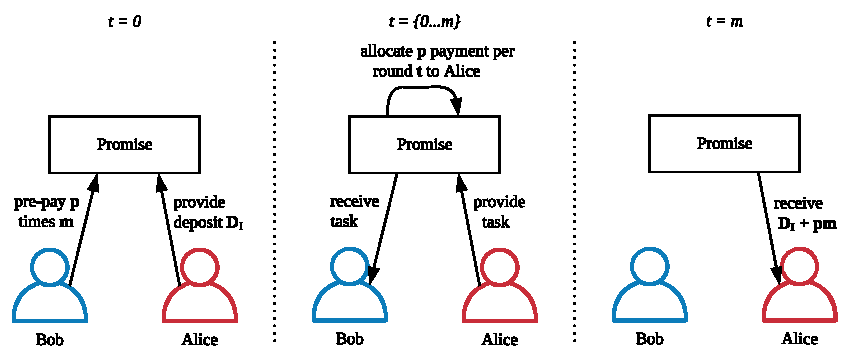
\includegraphics[width=\textwidth]{figures/protocol.pdf}
    \caption{\sys allows intermediaries (Alice) to lock less initial deposit $D_I$ and use payments $p_i$ provided by users (Bob) as additional deposit. The initial deposit and payments are locked until time $m$ determined by Bob. Only when Alice fulfills the specification $\Phi$ until $t=m$ can Alice withdraw her initial deposit $D_I$ and the total payments $pm$.}
    \label{fig:promise}
\end{figure}

\subsection{Protocol}

The \sys protocol consists of three steps.
We denote the service provider as $A$, the user as $B$, and the smart contract implementing \sys as $\mathrm{P}$.
We assume that $A$ and $B$ have agreed the total payment and the period over which the payment is to-be-paid in advance.

\begin{enumerate}
    \item At $t=0$: $B$ locks $m$ payments in $\mathrm{P}$. $A$ locks the initial deposit $D_I$ in $\mathrm{P}$.
    \item At $t=\{1, ..., m\}$: $A$ provides $m$ times the agreed task to $B$. $\mathrm{P}$ allocates one payment $p$ to $A$, if (i) $A$ provides a proof to $\mathrm{P}$ that fulfills the specification $\Phi$, or (ii) $B$ does not provide a fraud proof that $A$ did not provide the task within a determined time~\cite{Al-Bassam2018}.
    \item At $t=m$: $A$ withdraws $p(m+1)$ and $D_I$ from $\mathrm{P}$.
\end{enumerate}

To argue about the security of \sys, we introduce two concepts: (i) sequential-games with discounting and (ii) a likelihood of users exiting the system upon the service provider not adhering to the specification of the agreement.

\subsection{Sequential Games and Discounting}
Introducing \sys transforms the single-shot game of the agreement between Alice and Bob into a sequential-round game.
Instead of Alice and Bob treating each game in isolation, they need to consider the utilities for the sequence $m$ of the game.

\emph{Without} \sys, at each round $t$, Alice decides if she prefers to fulfill the specification based on the utilities denoted by Eq.~(\ref{eq:status-quo_alice}) and~(\ref{eq:status-quo_bob}).

\emph{With} \sys, Alice needs to consider that if she does not adhere to $\Phi$ in any round $t$, she does not receive any of the payments.
For example, if Alice provided the services according to $\Phi$ for $n$ rounds, but fails to do so in a round $t<m$, she does not receive $pn$ payments, but rather looses $D_I$ and receives $0$ payments.

Hence, Alice's decision needs to account for all $p \cdot m$ payments.
Furthermore, payments are made in the future.
A promised payment in the future is less valuable to Alice today, which we denoted with the parameter $\delta$.
$0<\delta<1$ denotes the discount factor of an agent's valuation of future utility. 
% Discounting captures the notion that the future is worth less than the present.
We argue that an agent can spend received payments somewhere else or potentially invest the payment for a profit.
% The potential profit of a monetary unit is encoded with $\mathrm{E}[r]$, as the expected rate of return.
Hence, the service provider faces an opportunity cost for delayed payments.
% because it is in the future.
% \rk{"because it is in the future" I really find this too much of a simplification.}
The payoffs to Alice, if she follows the same course of action over every round, are as follows. 

\begin{equation}
\label{eq:time_alice}
u_A(t) = 
\begin{cases}
    \sum_{t=0}^{m-1} \big( \frac{\delta}{1+r} \big)^{t} ( p - (t+1)\mathrm{E}[r]p -\mathrm{E}[r]D_{I}), & \text{if $\Phi=1$} \\
    % \big( \frac{\delta}{1+r} \big)^{m} pm - D_{I}((1+\mathrm{E}[r])^{m}-1), & \text{if $\Phi=1$} \\
    \sum_{t=0}^{m-1} \big( \frac{\delta}{1+r} \big)^{t} (V_A - \mathrm{E}[r]D_{I}-D_{I}), & \text{if $\Phi=0$} \\
\end{cases}
\end{equation}

% where 

% \begin{equation}
% \label{eq:status-quo_alice_cheat}

% \end{equation}

\noindent Bob receives the following pay-off, depending on Alice's behavior.

\begin{equation}
\label{eq:time_bob}
u_B (t) = 
\begin{cases}
    \sum_{t=0}^{m-1} \big( \frac{\delta}{1+r} \big)^t (V_B - p - c - (m-t)\mathrm{E}[r]p), & \text{if $\Phi=1$} \\
    \sum_{t=0}^{m-1} \big( \frac{\delta}{1+r} \big)^t (D_{I} - V_B - c) , & \text{if $\Phi=0$} \\
\end{cases}
\end{equation}


\subsection{Termination Probability}
Lowering Alice's initial collateral to $D_I$ increases the risk of Alice not fulfilling the specification of the agreement.
% As shown in Eq. (\ref{eq:time_alice}), Alice will misbehave if her payoff for cheating is higher than her provided collateral $D_I$ plus the sum of payment $pm$.
Specifically, in the first round, Alice's collateral is the lowest since she has not provided the service yet and has not added any payment into her collateral pool.
% \dom{Note for a later point: Lemma: Given a single-shot game between Alice and Bob. If Alice decides to cheat on Bob at $t=0$, then Alice cheats in all subsequent rounds on Bob.}
% By reducing her collateral we essentially promote cheating.
% However, we argue that in practice Bob would leave the protocol after a certain number of times he is being mistreated, \emph{if he has another choice}.
% Therefore, we introduce an exit probability $\beta$ for Bob.

% Eq. (\ref{eq:status-quo_alice}) and (\ref{eq:time_alice}) implicitly assume that Alice and Bob are playing a one-shot game ad infinitum.
% Under this framework, Bob would happily being tricked out of his $V_B$ again and again by Alice.
We argue that Bob exits a protocol after Alice not adhering to $\Phi$, encoded in the function $\beta(n) \to [0,1)$ describing the likelihood that Bob remains in the protocol.
The variable $n$ describes the number of times Bob tolerates Alice not delivering the service.
Each time Bob does not received $V_B$ due to Alice not providing the service as agreed, the lower the probability that Bob continues to participate.
Each user can have its own $\beta(n)$ function where users might choose to never participate with a service provider again, i.e., $\beta(1) = 0$ and others might tolerate a higher number of incidents.
This changes Alice's pay-off for the protocol as follows.
% Hence, if Alice considers $m$ rounds of the game, she receives the following payoffs:

\begin{equation}
\label{eq:beta_alice}
u_A(t) = 
\begin{cases}
    \sum_{t=0}^{m-1} \big( \frac{\delta}{1+r} \big)^{t} ( p - (t+1)\mathrm{E}[r]p -\mathrm{E}[r]D_{I}), & \text{if $\Phi=1$} \\
    %\big( \frac{\delta}{1+r} \big)^{m} pm - D_{I}((1+\mathrm{E}[r])^{m}-1), & \text{if $\Phi=1$} \\
    \sum_{t=0}^{m-1} \big( \frac{\delta}{1+r} \big)^{t} (\beta(n) V_A - \mathrm{E}[r]D_{I}-D_{I}), & \text{if $\Phi=0$} \\
\end{cases}
\end{equation}

% Bob's payoffs are as follows:
% \begin{equation}
% \label{eq:promise_bob}
% u_B (t) = 
% \begin{cases}
% \sum_{t=0}^{m} \big( \frac{\delta}{1+r} \big)^t (V_B - p - \mathrm{E}[r]p(m-t)) - c, & \text{if $\Phi=1$} \\
% \sum_{t=0}^{m} \big( \frac{\delta}{1+r} \big)^t \beta (D -V_B -c) , & \text{if $\Phi=0$} \\
% \end{cases}
% \end{equation}


As $\beta$ decreases, the payoff to Alice can become negative for not fulfilling the specification if $\beta(n) V_I < \mathrm{E}[r]D_I - D$.
For Alice, we increase the motivation to follow the specification by (i) providing a sum of payments $pm$ that Bob locks in the protocol, and (ii) the fear of Bob leaving the protocol altogether if she does not provide the service the entire period. % as expressed by $\frack{\beta}{n_c}$.
As Bob chooses $m$, he has a direct influence on Alice's expected pay-off.
By setting large $m$ and being able to quit the protocol upon Alice's misbehavior, he can motivate ``rational Alice" to act in his interest.
% for cheating converges to $0$, leaves Alice no other rational choice than to act honestly.
% Overall, Alice can join protocols with less initial collateral while providing Bob with the option to use ongoing payments as an additional security measure.
% For Alice, we can see that whether she behaves honestly or cheats, if $D_I+p=D$, her payoffs remain the same.
% However, the difference is that it is now easier for Alice to participate in the system and offer a service to Bob, since the deposit she has to provide, $D_I<D$. 
% For Bob, his utility is improved whether Alice is honest or cheats, since $c_L<C$.

%-------------------------------------------------
%---------------Security------------------------
%-------------------------------------------------

\section{Analysis}
\label{sec:security}

% We argue about the security of adding \sys to an existing protocol.
The core argument of \sys is that by locking multiple payments, service providers can reduce their initial collateral.
Specifically, introducing \sys to a protocol $\pi$, does not increase the incentive for an intermediary $A$ to not adhere to the specification.
This means that $\pi_{\mathrm{P}}$ and $\pi$ are equivalent in terms of security considering an economically rational intermediary $A$ under Def.~\ref{def:security}.
More formally, we state that:

\begin{theorem}[Security equivalence]
\label{thm:security}
Given a protocol $\pi$ that has a verifiable specification $\Phi$ and a economically rational service provider $A$ that provides more initial collateral $D_I$ than an incentive $V_A$ to violate the specification, introducing \sys is secure if $A$ does not gain additional utility by not fulfilling the specification considering $A$ participates in at least two rounds in $\pi$.
% Given an economically rational intermediary $A$ with a private valuation $V_A$ and an unknown termination probability $\beta$, a cryptoeconomic protocol with \sys, $\pi_{\mathrm{P}}$, is secure if $A$'s utility $u_A$ for behaving honest is higher than her utility for being malicious.  
\end{theorem}

\subsection{Action Choices}

Alice's utility for choosing a specific course of action i.e., fulfilling vs. not fulfilling the specification, is given by Eq.~(\ref{eq:beta_alice}).
However, this makes an implicit assumption: Alice considers the entire period $m$ as a basis for her decision.
We depict her added utilities for an example of two rounds in Fig.~\ref{fig:payoffstree}.

\begin{figure}[h!]
    \centering
    \resizebox{1\textwidth}{!}{
    \begin{forest}
    for tree={
    draw,
    font=\footnotesize,
    grow=east, 
    inner sep=0.5em, 
    s sep=0.1cm, 
    l sep=4.5cm,
    align=center, 
    edge={->, line width=1.5pt, color=blue},
    for children={fit=tight, anchor=base west}
    }
    [{$t=0$}, name=rootnode,
        [{$t=1$}, name=L2, edge label={node[midway,sloped,above,color=blue]{$p-\mathrm{E}[r]p-\mathrm{E}[r]D_I$}}
            [{$t=2$}, name=L3, edge label={node[midway,above,color=blue]{$\sum^1_0(\frac{\delta}{1+r})^t(p-\mathrm{E}[r]p-\mathrm{E}[r]D_I)$}}
            ]
        ]
    ]
    % \draw[->,color=blue, line width=1.5pt] (L3) to[out= north east,in=north west] node[below] {$\sigma_d$} node[above] {$p-c_A-\mathrm{E}[rD_3]$} (L3);
    \draw[->,dotted,color=red, line width=1.5pt] (L2) to[out=south east,in=south west] node[below] {$-\mathrm{E}[r]p-\mathrm{E}[r]D_I+(\frac{\delta}{1+r})(V_A-\mathrm{E}[rD_I]-D_I)$} (rootnode);
    % \draw[->,dotted,color=red, line width=1.5pt] (L3) to[out=south east,in=south west] node[above] {$\sigma_u$} node[below] {$v-c_A-\mathrm{E}[rD_3]-D_3$} (rootnode);
    \draw[->,dotted,color=red,line width=1.5pt] (rootnode) to[out=north east,in=north west] node[above] {$V_A-\mathrm{E}[rD_I]-D_I$} (rootnode);
    \end{forest}}
    % \vspace{-2em}
    \caption{Depicting the sum of utilities depending on different action choices made by Alice. At $t=0$ Alice can choose between fulfilling the specification and receive the utility depicted in blue or choose the opposite and receive the utility depicted in red. If Alice at any point prefers to violate the specification, the game restarts and the action choices are essentially back to the $t=0$ state. Furthermore, at $t=1$, Alice will already have committed to adhering to the specification. In case Alice decides to misbehave at this point, she will not receive $p$ that she was allocated when she transitioned to $t_1$. However, if she decides to continue to fulfill the specification, she will be rewarded with an additional payment allocation. This game continues until $t=m$.}
    %Payoffs corresponding to no action, $\sigma_p \in \emptyset$, are excluded as doing nothing would yield negative utility for an agent and therefore a rational agent would not choose this option.
    \label{fig:payoffstree}
\end{figure}

Showing that Thm.~\ref{thm:security} holds, requires considering that Alice might not participate for $m$ rounds.
Specifically, Alice might still consider the agreement as a single-shot game with a decision horizon of exactly one round.
Following this, we can use $m=1$ and Eq.~(\ref{eq:time_alice}) to conclude that Alice prefers to fulfill the specification if:

\begin{equation}
\label{eq:decision_promise_alice}
    p - \mathrm{E}[r]p > \beta(n) V_A - D_I
\end{equation}

\paragraph{Collateral Condition}
Comparing Alice's decision without \sys in Eq.~(\ref{eq:decision_model_alice}) and her decision with \sys in Eq.~(\ref{eq:decision_promise_alice}) without considering $\beta$ clearly shows that if Alice only considers a single round, introducing \sys \emph{weakens} the security of $\pi$ as Alice is not paid immediately and the initial collateral is reduced.
Moreover, even if Alice considers multiple rounds, if Eq.~(\ref{eq:decision_promise_alice}) does not hold, Alice \emph{has a higher utility to not fulfill the specification} if Bob is willing to continue to enter into agreements with her.
Even worse, if Bob decides to continue using the protocol $\pi$ and black-lists Alice for her violating $\Phi$, Bob still might end up with a Sybil identity of Alice.
Hence, for \sys to not weaken security the initial collateral needs to be set above $\beta(n)V_A-p+\mathrm{E}[r]p$.

In practice, this is achieved by over-collateralization or state-reversal.
Over-collateralization is used in XCLAIM where a vault has to provide 200\% collateral of the value it stands to obtain by violating the specification.
In NOCUST and, generally, payment channel networks, participants are not able to steal funds, since an older state can be committed that reverses the stealing of funds.


\subsection{Security Proof}

% We are now proving Thm.~\ref{thm:security}.

\begin{proof}
Under the assumption that $A$ is economically rational, wants to participate in at least two rounds, e.g. $t>0$, and Eq.~(\ref{eq:decision_promise_alice}) holds, we prove that $\pi_{\mathrm{P}}$ is secure.
If Eq.~(\ref{eq:decision_promise_alice}) holds, Alice should fulfill the specification in the first round.
We now show that if this holds, Alice should continue with the same course of actions in any subsequent round $t \in m$.
0375+
If if at any point $k \in m$, Alice decides to stop adhering to the specification she will receive the following pay-off:
\begin{equation}
    u_A(t,k) = \sum^{k-1}_{t=0} \big(\frac{\delta}{1+r} \big)^{t} (- (t+1)\mathrm{E}[r]p -\mathrm{E}[r]D_{I})+\big(\frac{\delta}{1+r} \big)^{t} (\beta(n) V_A - \mathrm{E}[r]D_{I}-D_{I})
\end{equation}
Alice has locked her collateral $D_I$ for multiple rounds as well as the payments she should have received.
Due to her actions she gains $V_A$ but for each round she has locked more payments and collateral, the higher her cost to change her choices of action w.r.t. the specification.
Moreover, if Alice plans to participate in multiple rounds, she stands to decrease her probability to provide services for other users depending on $\beta$.
Hence, assuming Alice is economically rational, Alice has the highest pay-off when fulfilling the specification until she has completed the service within the entire subscription period $m$, i.e., it is incentive compatible.
\end{proof}

\subsection{Cost Reduction for Service Providers}
Service providers can reduce their initial collateral to the lower bound under the condition of Eq.~(\ref{eq:decision_promise_alice}).
From this equation, we can determine the reduction if Alice only considers a single round of the game.
We express $D_I$ as $D - \rho$ where $\rho$ is the reduction of the initial collateral and solve for $\rho$
This yields:

\begin{equation}
    \label{eq:single_round_reduction}
    \rho = p - \mathrm{E}[r]p + D - \beta(n) V_A
\end{equation}

However, if we consider that Alice wants to participate in $m$ rounds, we can express this based on Eq.~(\ref{eq:beta_alice}) and solving for $\rho$.
However, we argue that under the assumption of Eq.~(\ref{eq:decision_promise_alice}), Alice's decision is essentially between participating a single round and not fulfilling the specification, or participating multiple rounds over the pre-agreed period $m$ while adhering to the specification.
To calculate Alice's decision bound, we are assuming that from Eq.~(\ref{eq:single_round_reduction}) the first reduction is set to the lowest possible value.
This means that the term $\beta(n)V_A - p + \mathrm{E}[r]p - D_I = 0$, i.e., at the decision bound Alice is undecided if she should fulfill the specification since the utilities for both choices are equal.
Thus, $\rho$ can be expressed as:
\begin{equation}
    \label{eq:multi_round_reduction}
    \rho = \sum_{t=0}^{m-1} \big( \frac{\delta}{1+r} \big)^{t} ( p - (t+1)\mathrm{E}[r]p - \mathrm{E}[r]D)
    % \rho =  \frac{\sum_{t=0}^{m-1} \big( \frac{\delta}{1+r} \big)^{t} ( p - t\mathrm{E}[r]p)  - V_A + D - \sum_{t=1}^{m-1} \big( \frac{\delta}{1+r} \big)^{t} \mathrm{E}[r]D}{1 - \sum_{t=1}^{m-1} \big( \frac{\delta}{1+r} \big)^{t} \mathrm{E}[r]}
\end{equation}

In Section~\ref{sec:xclaim} we give an example how collateral is lowered given a set of parameters.
Note that to calculate the collateral reduction, both the service provider and the user only need to know the prior collateral requirement $D$ as defined by $\pi$.
For example, in XCLAIM this is 200\%.


% \begin{equation}
%     \label{eq:multi_round_reduction}
%     \rho = \sum^{m-1}_{t=0} \big(\frac{\delta}{1+r} \big)^{t} (p - t\mathrm{E}[r]p -\mathrm{E}[r]D_{I}) + D - V_A
% \end{equation}


% \sys ensures that funds are secure. 
% Payments $p$ (future and current) provided by a user as well as deposits $D$ by intermediaries cannot be stolen. This property is fulfilled by implementing the escrow as a smart contract on a ledger with a functionality and appropriate security parameters as described in~\cite{garay2016bitcoin,gervais2016security}. 
% Apart from this, \sys aims to fulfil the following properties:

% \begin{enumerate}
%     \item \textbf{Security equivalence}: Given Def.~\ref{def:security}, introducing \sys to a protocol $\pi$, does not increase the incentive for an intermediary $A$ to behave malicious.
%     \item \textbf{Sybil resistance}: Alice cannot increase her pay-off $u_A$ by creating multiple Sybil identities $A'$.
% \end{enumerate}



% \subsection{Security equivalence}

% We argue that $\pi_{\mathrm{P}}$ and $\pi$ are equivalent in terms of security considering an economically rational intermediary $A$.



% To prove Theorem~\ref{thm:security}, we consider both action choices of Alice.
% Given Eq.~(\ref{eq:promise_alice}), Alice has different payoffs depending on her being honest or malicious.
% We can calculate the decision bound for Alice's individual rational choice to cheat Bob by comparing the two options.
% \begin{equation}
% \label{eq:decision-bound-alice-full}
%      \sum_{t=0}^{m} \big( \frac{\delta}{1+r} \big)^{t} ( p - t\mathrm{E}[r]p -\mathrm{E}[r]D_{I}) = 
%     \sum_{t=0}^{m} \big( \frac{\delta}{1+r} \big)^{t} \beta (V_A - \mathrm{E}[r]D_{I}-D_{I})
% \end{equation}

% Using Eq.~(\ref{eq:decision-bound-alice-full}) above, we can determine a decision bound based on the $\beta$ function of Alice to behave honestly.
% The $\beta$ function, in turn, determines how large the initial deposit $D_I$ needs to be to prevent Alice from cheating.

% \begin{proof}
% Assume $A$ is individually rational, $A$ will choose an action based on the highest pay-off.
% We re-arrange Eq.~(\ref{eq:decision-bound-alice-full}) for $\beta$:
% \begin{align}
%     \label{eq:decision-bound-beta}
%     \beta = \frac{\sum_{t=0}^{m} \big( \frac{\delta}{1+r} \big)^{t} ( p - t\mathrm{E}[r]p -\mathrm{E}[r]D_{I})}{\sum_{t=0}^{m} \big( \frac{\delta}{1+r} \big)^{t} (V_A - \mathrm{E}[r]D_{I}-D_{I})} 
% \end{align}
% From Eq.~(\ref{eq:promise_alice}), we can notice that the smaller $\beta$ becomes, the smaller the pay-off for being malicious for $A$ becomes.
% Hence, if $\beta \to 0$, $A$ has no incentive to be malicious and should behave honest.
% However, if $\beta \to 1$, Alice's incentive to be malicious is largely determined by the $V_A-\mathrm{E}[r]D_I - D_I$ term.
% Further, we can clearly see that at $\beta=1$, Eq.~(\ref{eq:decision-bound-beta}) and Eq.~(\ref{eq:time_alice}) are equivalent.
% From this follows that if $\beta \to 1$ then the initial deposit locked must also approach the deposit locked as without \sys, i.e., $D_I \to D$.
% As long as $\beta$ and $D_I$ are set such that the utility for $A$ to behave honestly is greater, a protocol implying \sys is considered secure.
% \end{proof}


% Of course, $A$ has an interest to lower the initial deposit $D_I$, so it is hard for the user to determine if $D_I$ is set adequately.
% In a practical setting, for example in payment channels or commit-chains, $D_I$ can be set to exactly the value $V_B$ that the user associates with the task.
% The additional payments can then be used to increase the amount of transactions that can be made through the payment channel or the amount of assets that can be finalized via the commit-chain.


% We can re-arrange this equation to determine $\beta$:
% \begin{equation}
%     \label{eq:beta}
%     \beta = \frac{\big( \frac{\delta}{1+r} \big)^{m} pm - D_{I}((1+\mathrm{E}[r])^{m}-1)}{\sum_{t=0}^{m} \big( \frac{\delta}{1+r} \big)^{t} (V_A - \mathrm{E}[r]D_{I}-D_{I})}
% \end{equation}
% 

% \subsection{Sybil Resistance}

% Alice reduces her initial collateral with \sys.% from $D$ to $D_I$ where $D_I < D$.
% While this lowers her entry barrier, arguably this makes it easier for Alice to cheat in the protocol as she has less at stake.
% By introducing $\beta$ we Alice's desire to cheat is reduced.
% More formally, 
%We can calculate the decision bound for Alice's individually rational choice to cheat Bob by comparing the two options in Eq. (\ref{eq:promise_alice}).
% \begin{equation}
%     \big( \frac{\delta}{1+r} \big)^{m} pm - D_{I}((1+\mathrm{E}[r])^{m}-1) =
%     \sum_{t=0}^{m} \big( \frac{\delta}{1+r} \big)^{t} \beta (V_A - \mathrm{E}[r]D_{I}-D_{I})
% \end{equation}
%We can re-arrange this equation to determine $\beta$:
%\begin{equation}
%    \label{eq:beta}
%    \beta = \frac{\big( \frac{\delta}{1+r} \big)^{m} pm - D_{I}((1+\mathrm{E}[r])^{m}-1)}{\sum_{t=0}^{m} \big( \frac{\delta}{1+r} \big)^{t} (V_A - \mathrm{E}[r]D_{I}-D_{I})}
%\end{equation}
% \dom{re-arrange for $\beta$}

%Similarly, Bob can determine how high $D_I$ should be under the assumption that he knows $V_A$ and the parameters $r$ and $\delta$.

% \dom{re-arrange for $D_I$}
%\begin{equation}
%    \label{eq:d_initial}
%    D_I = \frac{\big( \frac{\delta}{1+r} \big)^{m} pm - \sum_{t=0}^{m} \big( \frac{\delta}{1+r} \big)^{t} \beta V_A}{ ((1+\mathrm{E}[r])^{m}-1) - \sum_{t=0}^{m} \big( \frac{\delta}{1+r} \big)^{t} \beta (\mathrm{E}[r]-1)}
%\end{equation}

%Assuming that $\beta$ is lowered aggressively, i.e.\ Bob tolerates only few task violations $n_c$, Alice  chooses to be honest as this maximizes her payoff.
% Being honest with a reduced collateral $D_I$ is thereby the individually rational choice.
% Given that Bob is aware for the involved parameters $V_A$, $r$, and can set the parameters $p$ and $m$ himself, Bob is able to calculate at which likelihood he should exit a given protocol given by Eq. (\ref{eq:beta}).
% Similarly, Bob can decide which level of colalteral $D_I$ is sufficent for him using Eq.(\ref{eq:d_initial}).

% \subsection{Sybil resistance}
%\subsubsection{Sybil Identities}
% We argue that if $\beta$ is lowered aggressively, Alice can do no better than being honest.
% However, if there is a non-negligible probability that Bob remains in the protocol after being cheated once, Alice can try to create a Sybil identity $A'$ to (i) cheat Bob in round $t=0$ and (ii) behave honestly in round $1$ to $m+1$.
% Hence, Bob can only be sure to prevent Alice from executing a Sybil attack, if $\beta = 0$.

% \subsection{$\beta$ Factor Over Time}
% The $\beta$ factor set by Bob is the crucial security parameter for Bob given we are in a permissionless system.
% We argue that setting the $\beta$ factor depends on Bob's reliance on participating in a protocol with a specific intermediary.
% If Bob \emph{requires} the service Alice provides and there is \emph{no alternative} within the same protocol in which Alice operates, Bob is faced with a \emph{monopoly}.
% In a monopoly Bob $\beta$ likely never approaches 0 as Bob is forced to tolerate Alice's misbehavior.
% To protect Bob, \sys requires that $D_I$ of Alice is close or equal to $D$ in a monopoly.
% % Otherwise, Alice can create Sybil attacks on Bob or just outright cheat every round as Bob would try to use the service over and over.

% The opposite market situation is \emph{perfect competition}.
% Bob can choose from a wide selection of service providers to interact with\footnote{
% However, as we lack strong identities, these service providers could all be Sybil identities of Alice.
% Recognizing that perfect competition exists is a challenging task and we leave this as future work.}.
% Assuming perfect competition exists, Bob has the choice to pick another intermediary any time.
% As an example, we could imagine Bob choosing between several operators in NOCUST or vaults in XCLAIM.
% If Bob would be cheated on by an intermediary in NOCUST, he could switch to using another ooperator.
% In turn, Bob can set $\beta$ to 0.
% In these cases, we can substantially lower the initial collateral $D_I$ using Eq. (\ref{eq:decision-bound-beta}).


% \section{Economic Benefits}
% \label{sec:benefits}

% \begin{enumerate}
%     \item \textbf{Cost reduction for users}: Bob is able to reduce transaction costs $c$ by paying for multiple rounds $m$ of services for payment $p$ in advance.
%     \item \textbf{Collateral reduction for intermediaries}: Alice is able to provide a lower deposit $D_I$ than the deposit required in a single-shot game setting $D$ while Bob enjoys the same level of security against Alice.
% \end{enumerate}

% \subsection{Security of funds}
% Both Alice and Bob store their funds in escrow.
% The escrow needs to be securely implemented as a smart contract.
% % As such, funds are secure given that the underlying ledger functionality is secure.
% The \sys smart contract is required to monitor the status of the service provided by Alice to Bob, such that any potential safety or liveness failure in the target protocol is detected, and any locked payments held in escrow by the contract are released to Bob upon detection. If no failures are detected during the pre-agreed period, the smart-contract allows Alice to withdraw her earned payments.

% The security of operations performed in this smart contract is determined by the guarantees of the underlying ledger. Extensive discussion of this is outside the scope of this paper and we refer the reader to~\cite{garay2016bitcoin,gervais2016security}. We assume in our work that the safety or liveness provisions of the underlying ledger are not violated. %is operated by an honest majority such that no .

\subsection{Cost Reduction for Users}
Assume that Alice behaves honestly.
If a user pays every round $t$ for the service provided by Alice, then his pay-off per round is $V_B - p - c$ as described in Eq. (\ref{eq:status-quo_bob}). % where $V_B$ is his private value for getting the service, $p$ the payment he makes and $c$ the cost for doing the payment.
However, locking multiple payments incurs opportunity cost.
This cost is lowered at every time step as the payments are assigned to the intermediary, as expressed in Eq.~(\ref{eq:time_bob}).

Bob starts with an opportunity cost of $\mathrm{E}[r]pm$ at $t=0$. 
The opportunity cost is reduced to $\mathrm{E}[r]p(m-1)$ at $t=1$ as the payment is allocated to Alice.
Generalizing this for $t$ rounds, leaves us with $\mathrm{E}[r]p(m-t)$ at every time step $t$ from today's perspective.

The user locks future payments when the sum of the transaction costs $c$ for $m$ payments is greater than the opportunity cost for locking additional payments plus the single transaction cost for making the prepayments.
Hence, the boundary for a user to choose \sys as individually rational choice maximizing his pay-off is given by:

\begin{align}
    \sum_{t=1}^m \big( \frac{\delta}{1+r} \big)^t c = \sum_{t=0}^m \big( \frac{\delta}{1+r} \big)^t \mathrm{E}[r]p(m-t)
\end{align}
\begin{align}
\label{eq:decision-bound-user}
c = \mathrm{E}[r]p(m-t)    
\end{align}

Provided the right hand of Eq. (\ref{eq:decision-bound-user}) is smaller, Bob should use \sys to lock multiple payments $pm$ as it is his individually rational choice that maximizes his pay-off $u_B$.







%-------------------------------------------------
%---------------APPLICATION------------------------
%-------------------------------------------------


\section{Applications}
\label{sec:application}

In this section we apply \sys to the XCLAIM protocol.
We show analytically how \sys is able to reduce the initial amount of locked deposits.
Further, we give a sketch how \sys can be implemented in NOCUST.
% \aza{Shorten this to 1 paragraph and rather add 2 more applications! For the paper, it is better to even have a single paragraph, but highlight multiple protocols - rather than going into detail on 1 specific.}

\subsection{XCLAIM}
\label{sec:xclaim}

XCLAIM is a protocol that allows users to transfer assets between heterogeneous decentralized ledgers using a collateralized service provider called a vault~\cite{Zamyatin2019XCLAIM}.
Instead of relying on a trusted third party like a centralized exchange, the vault must provide collateral to ensure that it does not steal the coins it holds in custody.
It has to verify correctness of her actions by submitting transaction inclusion proofs to the smart contracts that augments the protocol.
\sys can be applied such that the vault, Alice, locks some initial collateral $D_I$ and issues backed-tokens using this collateral.
Bob, using the service, is able to lock the future payments of Alice to allow him to transfer more assets between the ledgers.

\paragraph{Initial Parameters}
XCLAIM uses an initial set of parameters as follows:
\begin{itemize}
    \item Initial Collateral $D$: A service provider needs to provide 200\% collateral $D$ in comparison to the value held in custody $V_A$.
    \item Payments $p$: Although payments are not specified in the original XCLAIM paper, similar services such as tBTC require users to pay 0.9375\% of fees as payment\footnote{Based on \url{https://docs.keep.network/tbtc/index.pdf} from 3 May 2020.}.
    \item Rate of return $r$: A service provider needs to lock collateral in the ETH currency to participate. Possible alternatives offer a maximum of 3.75\% APR rates\footnote{Based on \url{https://www.coingecko.com/en/earn/ethereum} from 3 May 2020.}.
    \item Discount factor $\delta$: Service providers can discount future payments. As the price of cryptocurrencies is relatively volatile we adopt a strongly discounted future income at $0.75$ from~\cite{Harz2019Balance}.
\end{itemize}


\paragraph{Integrating Promise}
For sake of example, we are using BTC as the issuing currency and ETH as the backing currency.
This means that the vault, the service provider, has to lock ETH as collateral to provide security against stealing BTC it holds in custody.
Given the parameters, \sys can be integrated as follows.
\begin{enumerate}
    \item The user and a vault agree on a subscription period $m$. For example, the user and the vault can agree that the vault will be responsible for the next ten Bitcoin-backed tokens issued or redeemed by this users that are each 1 BTC in size.
    \item The user and the vault set-up a \sys contract in which the user pre-pays $m=10$ fees at 0.9375\% of 1 BTC for the next ten requests at a set price of $p=0.009375$ to issue or redeem Bitcoin-backed tokens.
    \item The vault then deposits the initial deposit $D_I$ into the contract.
    \item Each time the user issues or redeems tokens with the vault, the vault is allocated a part of the payment $p$.
    \item Finally, after ten requests have been made, the vault can withdraw $pm$ and $D_I$.
\end{enumerate}

\paragraph{Cost Reduction}
For simplicity, we are going to denote all monetary amounts in BTC.
In XCLAIM, a vault would have to provide the equivalent of 2 BTC in collateral to hold custody over 1 BTC in value.
First, we calculate the possible $D_I$ collateral given Eq.~(\ref{eq:single_round_reduction}).
This gives us the minimum collateral required to also protect against a \textit{vault that plays a single-shot game}.
For simplicity, we are assuming that the vault has an incentive of 1 to steal the BTC (the current value of the Bitcoin) as well as a hidden motivation to steal BTC such that $V_A = D = 2$.
Moreover, the vault is not interested in any future collaboration with the user, hence $\beta(n) = 1$.
Last, we divide the 3.75\% APR through 365 days to get the average return.

\begin{equation}
\begin{split}
    \rho &= p - \mathrm{E}[r]p + D - \beta(n) V_A\\
    \rho &= 0.009375 - \frac{0.0375}{365} 0.0093750 + 2 - 2\\
    \rho &= 0.00937404
\end{split}
\end{equation}

Second, we are using Eq.~(\ref{eq:multi_round_reduction}) to explore the reduction factor $\rho$ if the \textit{vault plays a sequential game}.
Note that, at a minimum, a vault has at least a private value of $V_A$ to not follow the specification of XCLAIM: if the vault can take the 1 BTC and is punished with less collateral $D_I$ being taken away, it is incentive compatible for the vault to take the 1 BTC. Using the example values above, we calculate $\rho$ as:

\begin{equation}
\begin{split}
\rho &= \sum_{t=0}^{9} \big( \frac{\delta}{1+r} \big)^{t} ( p - (t+1)\mathrm{E}[r]p - \mathrm{E}[r]D) \\
\rho &= \sum_{t=0}^{9} \big( \frac{\delta}{1+r} \big)^{t} ( 0.009375 - (t+1)\frac{0.0375}{365}0.009375 - \frac{0.0375}{365}*2)
\end{split}
\end{equation}

\begin{figure}[t]
    \centering
    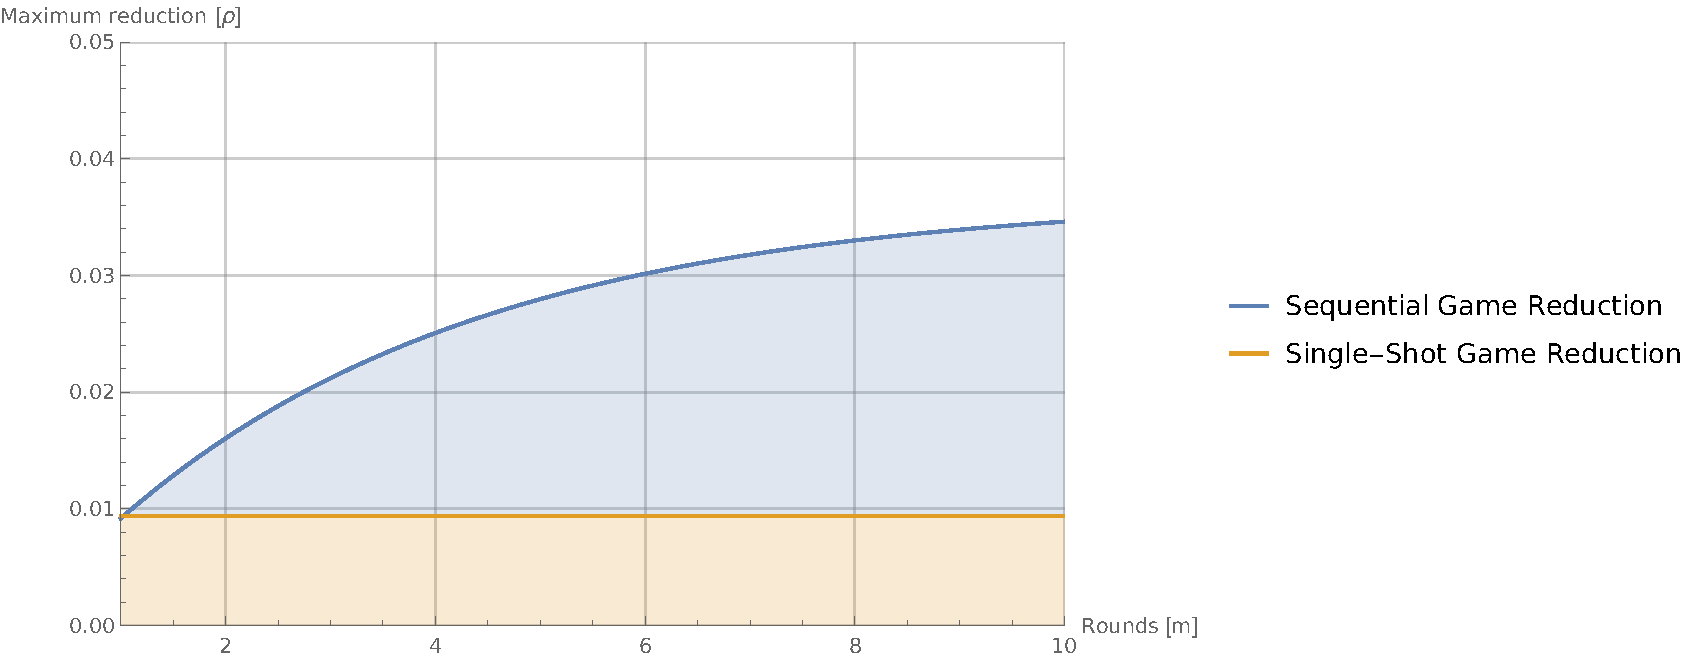
\includegraphics[width=\textwidth]{promise/figures/collateral-reduction.pdf}
    \caption{Caption}
    \label{fig:collateral}
\end{figure}

% \dom{
% \begin{itemize}
%     \item Calculate much initial collateral neds to be locked by Alice and how much assets can be transferred by Bob by the end of the period if Bob prepays amount $pm$.
%     \item Show a small figure that indicates that the locking period increases the chances of payments in subsequent rounds for Bob.
% % \end{itemize}
% }

\subsection{NOCUST}

NOCUST is a second-layer payment protocol whereby an untrusted intermediary operates a commit-chain to facilitate payments between its users~\cite{Khalil2019NOCUST}.
The application of \sys to NOCUST follows a similar approach as the XCLAIM example.
Hence, we are only giving a sketch of \sys's applicability here.

We consider a scenario where Alice is the intermediary commit-chain operator, and Bob is a payment recipient. In this setting we propose to employ \sys as follows: Any fee to be paid by Bob to Alice in exchange for the delivery of an incoming payment would be locked as collateral that Bob could claim if the NOCUST protocol fails. Over time, the fees locked in \sys would grant Bob instant finality over larger payments, increasing the utility of the service.
% We consider a scenario where Alice is the intermediary commit-chain operator, and Bob is a payment recipient. Alice can effectively deliver payments from other users to Bob without Alice having to put up additional collateral. However, without collateral, Bob has to wait for two rounds of the protocol to succeed before being guaranteed finality of an incoming payment. This delay in finality may be too long for certain use cases. 

% Using NOCUST with additional collateral by Alice, however, can provide instant finality for Bob. In this case, Alice puts up an amount of collateral that is equal to what Bob expects to receive within two rounds of the protocol, such that if the protocol fails and pending payments are reverted, the collateral put up by Alice can act as a reimbursement for any expenses Bob may have incurred before finalization. 

For example, in a sales scenario, Bob could release some goods immediately after Alice promises to deliver the payment for them, instead of waiting two rounds for guaranteed finality. If Alice fails to deliver the payment, her collateral would paid to Bob to cover the cost of the goods.

% In this setting we propose to employ \sys as follows: Any fee to be paid by Bob to Alice in exchange for the delivery of an incoming payment would be locked as collateral that Bob could claim if the NOCUST protocol fails. This gradually increases how reliable Bob perceives Alice to be as an intermediary as more fees are accumulated towards reimbursing Bob for any potential damages. If Bob wishes to utilize Alice's service with minimal risk, Bob would not release any goods in return for incoming payments until Bob is guaranteed finality. Over time, the fees locked in \sys would grant Bob instant finality over larger payments, increasing the utility of the service.

% \subsection{TrueBit}
% TrueBit is a protocol in which a set of intermediaries provide computation services~\cite{teutsch2017scalable}.


% \subsection{Dai stablecoin}

% Dai is a stablecoin in which intermediaries provide collateral to open so-called Collateralized Debt Positions (CDPs)~\cite{Maker2017Dai}.
% The collateral serves as a backing mechanism to ensure that the price of 1 Dai equals 1 USD.

\subsection{Implementation}

We implement \sys in Solidity in around 100 lines of code.
We use the implementation to experimentally assess the cost of executing the contract functions.
Our cost calculations are summarized in Table~\ref{tab:implementation} based on an Ether exchange rate of USD 172.61 and 1.5 Gwei gas price.
The implementation is available as an open source project\footnote{\url{https://github.com/nud3l/Promise/tree/master/src}}.

\begin{table}[h]
\centering
\caption{Overview of \sys functions and their cost.}
\label{tab:implementation}
\begin{tabularx}{\textwidth}{lXll}
\toprule 
\textbf{Function} & \textbf{Description} & \textbf{Gas cost} & \textbf{Cost} \\ \toprule
create & Setup function. & 112196 & USD 0.02895 \\ 
deposit & Called by intermediary to provide deposit. & 43291 & USD 0.01116 \\
payment & Called by user to provide pre-payment. & 43770 & USD 0.0113 \\ \midrule
deliver & Called as part of task provision. & 50703 & USD 0.01309 \\ \midrule
withdraw & Called by intermediary after the service period is up to receive payment and deposit. & 31788 & USD 0.0082 \\
\bottomrule
\end{tabularx}
\end{table}



%-------------------------------------------------
%---------------RELATED WORK------------------------
%-------------------------------------------------

\section{Related Work}
\label{sec:related}


% Relate to finance.

% \tolgu{Add related work from finance. The principle of pre-payment is not new, but only with smart contracts we can actually provide some guarantees that the funds will be returned to the users in if there is no misbehavior, i.e. cannot be stolen.}

There are two strands of related literature.
The first one comes from the financial world covering (advance) payments for financial contracts.
The second strand comes from the more recent work in decentralized ledgers.
In the economics literature, a wide range of work focuses on secured debt, such as ~\cite{scott1977bankruptcy,stulz1985analysis}.
However, these concepts rely on trust on third parties to maintain security in the debt and payment positions.
\sys replaces this third-party trust by holding advance payments in a smart contract escrow.
%which shows that some profitable projects will not be undertaken by a firm which can finance them only with equity or unsecured debt, but will be undertaken by a firm which can finance them with secured debt.
% \cite{boot1994moral} considers moral hazard and secured lending in the context of an infinitely repeated credit market game. 
% In addition, the issuance of secured debt has been argued to increase the value of a firm~\cite{scott1977bankruptcy}.
% Other work focuses on the efficiency secured debt under conditions of imperfect information~\cite{triantis1992secured}.
% Another branch of work relates to down payments (a payment made for something bought on credit)~\cite{engelhardt}. 
% ,mayer1996gifts,engelhardt1994house
%of secured debt~\cite{hill2001secured}, and 

On the second strand, Balance is a protocol that allows intermediaries to lower their collateral over time~\cite{Harz2019Balance}.
It operates at the other end of \sys: instead of lowering the initial collateral, the more an agent behaves honestly, the higher the reduction of collateral.
Balance requires the highest collateral to be provided at the start of the interaction between agents and makes the assumption that payments are close to 0 (i.e.,\ there is perfect competition).
\sys and Balance can be combined together to first reduce initial collateral when bootstrapping a new protocol and then lower collateral requirements for established agents over time.
Teutsch et al. discuss bootstrapping a token for verifiable computations~\cite{Teutsch2019Boostrap}.
This work discusses how to enable users, like Bob, to obtain the required funds to participate in TrueBit.
Their proposal includes a governance game that allows to exchange special governance tokens into collateral tokens (for intermediaries) and utility tokens (for users).
Lastly, the idea of bundling payments together is also introduced in~\cite{Berg2018} to create subscriptions for services of agents.
\sys extends this idea to allow collateral reduction for intermediaries.

% Other related work?
% \todom{Can you cover this? Does not have to be much, we have limited space.}
% \begin{itemize}
%     \item Balance
%     \item New paper by Teutsch
%     \item Payment streaming \url{https://github.com/ethereum/EIPs/issues/1620}
% \end{itemize}

%-------------------------------------------------
%---------------CONCLUSION------------------------
%-------------------------------------------------

\section{Conclusion}
\label{sec:conclusion}

We present \sys, a subscription mechanism that allows users to lock payments for future services for a period of time.
The locked payments are added to the initial collateral of a service provider, Alice, each time a service is delivered.
The core assumption for the security of \sys is that a user Bob is able to lock a number of payments up front and exit the protocol when Alice misbehaves receiving back all of his payments over the subscription period and the initial collateral provided by Alice.
On the other hand, Alice is able to utilize Bob's future payments as collateral throughout the subscription period.
% This allows Alice to reduce her initial collateral requirement, allowing protocols that adopt \sys to lower the burden on intermediaries.
% Bob is able to reduce his transaction cost as he transfers a sum of payments.
% Further, Bob is able to receive the service in full --- for the entire period he pre-paid --- or he is refunded the entire sum of payments.
We have introduced a semi-formal model for \sys.
We discuss the security and the effect of the $\beta$ parameter, but leave formal proofs of the security properties as future work.
We have shown how \sys can be applied to the XCLAIM protocol and shown a sketch of appliying it to NOCUST.

\section*{Acknowledgements}
The authors would like to thank Arthur Gervais and William Knottenbelt for their helpful feedback on this paper. Further, the authors thank the anonymous reviewers for their excellent feedback and suggestions for improvement.

\bibliographystyle{splncs04}
\bibliography{bib/blockchain,bib/references}

% \appendix

% \section{Decision Boundary}
% \label{app:decision-bound}

% We determine the decision boundary for the cost reduction parameter $\rho$ from Eq.~(\ref{eq:beta_alice}):


% \begin{equation}
% \begin{split}
%     \sum_{t=0}^{m-1} \big( \frac{\delta}{1+r} \big)^{t} ( p - t\mathrm{E}[r]p -\mathrm{E}[r]D_{I}) &= V_A - \mathrm{E}[r]D_{I}-D_{I}  \\
%     \sum_{t=0}^{m-1} \big( \frac{\delta}{1+r} \big)^{t} ( p - t\mathrm{E}[r]p -\mathrm{E}[r](D-\rho)) &= V_A - \mathrm{E}[r](D-\rho)-D+\rho \\
%     \sum_{t=0}^{m-1} \big( \frac{\delta}{1+r} \big)^{t} ( p - t\mathrm{E}[r]p) - V_A + D &= \rho - \mathrm{E}[r](D-\rho) + \sum_{t=0}^{m-1} \big( \frac{\delta}{1+r} \big)^{t} \mathrm{E}[r](D-\rho) \\
%     \sum_{t=0}^{m-1} \big( \frac{\delta}{1+r} \big)^{t} ( p - t\mathrm{E}[r]p)  - V_A + D  &= \rho + \sum_{t=1}^{m-1} \big( \frac{\delta}{1+r} \big)^{t} \mathrm{E}[r](D-\rho) \\
%     \sum_{t=0}^{m-1} \big( \frac{\delta}{1+r} \big)^{t} ( p - t\mathrm{E}[r]p)  - V_A + D - \sum_{t=1}^{m-1} \big( \frac{\delta}{1+r} \big)^{t} \mathrm{E}[r]D &= \rho - \sum_{t=1}^{m-1} \big( \frac{\delta}{1+r} \big)^{t} \mathrm{E}[r]\rho \\
%     \frac{\sum_{t=0}^{m-1} \big( \frac{\delta}{1+r} \big)^{t} ( p - t\mathrm{E}[r]p)  - V_A + D - \sum_{t=1}^{m-1} \big( \frac{\delta}{1+r} \big)^{t} \mathrm{E}[r]D}{\rho} &= 1 - \sum_{t=1}^{m-1} \big( \frac{\delta}{1+r} \big)^{t} \mathrm{E}[r] \\
%     \frac{\sum_{t=0}^{m-1} \big( \frac{\delta}{1+r} \big)^{t} ( p - t\mathrm{E}[r]p)  - V_A + D - \sum_{t=1}^{m-1} \big( \frac{\delta}{1+r} \big)^{t} \mathrm{E}[r]D}{1 - \sum_{t=1}^{m-1} \big( \frac{\delta}{1+r} \big)^{t} \mathrm{E}[r]} &= \rho  \\
% \end{split}
% \end{equation}

\end{document}
